\documentclass{article}

\usepackage{amsmath} % math stuff
\usepackage{amssymb} % math stuff
\usepackage{array} % equations and stuff
\usepackage{bm} % bold math
%\usepackage{booktabs} % extra table rule options
%\usepackage{caption} % suppressed table numbering; incompatible with revtex, and longtable, I think
\usepackage{comment} % comment environment
%\usepackage{enumitem} % customization of enumeration, itemize, and description
\usepackage[T1]{fontenc} % font encoding for special characters, must also use scalable font package
\usepackage[margin=0.8in]{geometry} % paper sizes and margins (but be careful not to mess up pre-defined pages)
\usepackage{graphicx} % for graphics
%\usepackage{helvet} % default font is the helvetica postscript font
\usepackage[utf8]{inputenc} % special characters in tex input
\usepackage{layouts} % print units like widths
\usepackage{lipsum} % lorem ipsum filler text
\usepackage{lmodern} % scalable font?
\usepackage{longtable} % multi-page tables
\usepackage{makecell} % specify line-breaks in table cells
\usepackage{mathrsfs} % math script font
\usepackage{mhchem} % easier chemical formula
\usepackage{microtype} % allows disabling of ligatures
\usepackage{multicol} % multicolumns
%\usepackage{newcent} % new century schoolbook font
\usepackage{nicefrac}
\usepackage{numprint} % print and format (large) numbers
\usepackage{parskip} % removes paragraph indentation, and adjusts paragraph skip, as well as list items
\usepackage{pdfpages} % add pdf files as pages
%\usepackage{setspace} % adjust text spacing and indents
\usepackage{siunitx} % decimal alignment
\usepackage{subfigure} % divided figures
%\usepackage{tabu} % extra table options
\usepackage{textcomp} % symbols
\usepackage{threeparttablex} % better footnotes with longtable
\usepackage{titling} % title placement
\usepackage{ulem} % strikethrough text
%\usepackage{url} % superceded by hyperref
\usepackage{verbatim} % verbatim environment
\usepackage{xcolor} % colors and color boxes
\usepackage{xspace} % commands that don't eat up white space
\usepackage{hyperref} % links and page setup; should always come last

\hypersetup{
 bookmarks=true,
 colorlinks=true,
 citecolor=blue,
 linkcolor=blue,
 urlcolor=blue,
 pdfstartview={XYZ null null 1.0} % default open view is 100%
}

\DisableLigatures[f,t]{encoding = T1} % disable ff, fi, fl, tt ligatures; without options, it also disables -- = endash
\renewcommand{\arraystretch}{1.1} % extra vertical (and horizontal?) space in tables

% define centered, left- and right-aligned columns with specified widths
\newcommand{\PreserveBackslash}[1]{\let\temp=\\#1\let\\=\temp}
\newcolumntype{C}[1]{>{\PreserveBackslash\centering}p{#1}}
\newcolumntype{L}[1]{>{\PreserveBackslash\raggedright}p{#1}}
\newcolumntype{R}[1]{>{\PreserveBackslash\raggedleft}p{#1}}

\begin{document}

\pagestyle{empty} % don't number pages

% custom title
\begin{center}
{\LARGE Express Riddler}

\vspace{0.15in}

{\Large 6 August 2021}
\end{center}


\section*{Riddle:}

I have four equilateral triangles.
I place one on the floor.
I pick a random edge of this first triangle and attach it to a side of a second triangle.
Next, I randomly pick one of the four edges of the resulting rhombus and attach the third triangle.
Finally, I randomly pick an edge from along the perimeter of the resulting shape and attach the fourth triangle.

What is the probability that I can create a regular tetrahedron by folding the four triangles along their edges?

\textit{Extra credit}: Instead of using four equilateral triangles to make a tetrahedron, suppose I use six squares to make a cube.
What is the probability I can make a cube by randomly attaching the squares, one at a time?
(And what are my chances of making any of the three other Platonic solids using their respective faces?)


\section*{Solution:}

The first three triangles will always attach to form the same shape (up to some rotation):

\vspace{0.1in}
\begin{center}
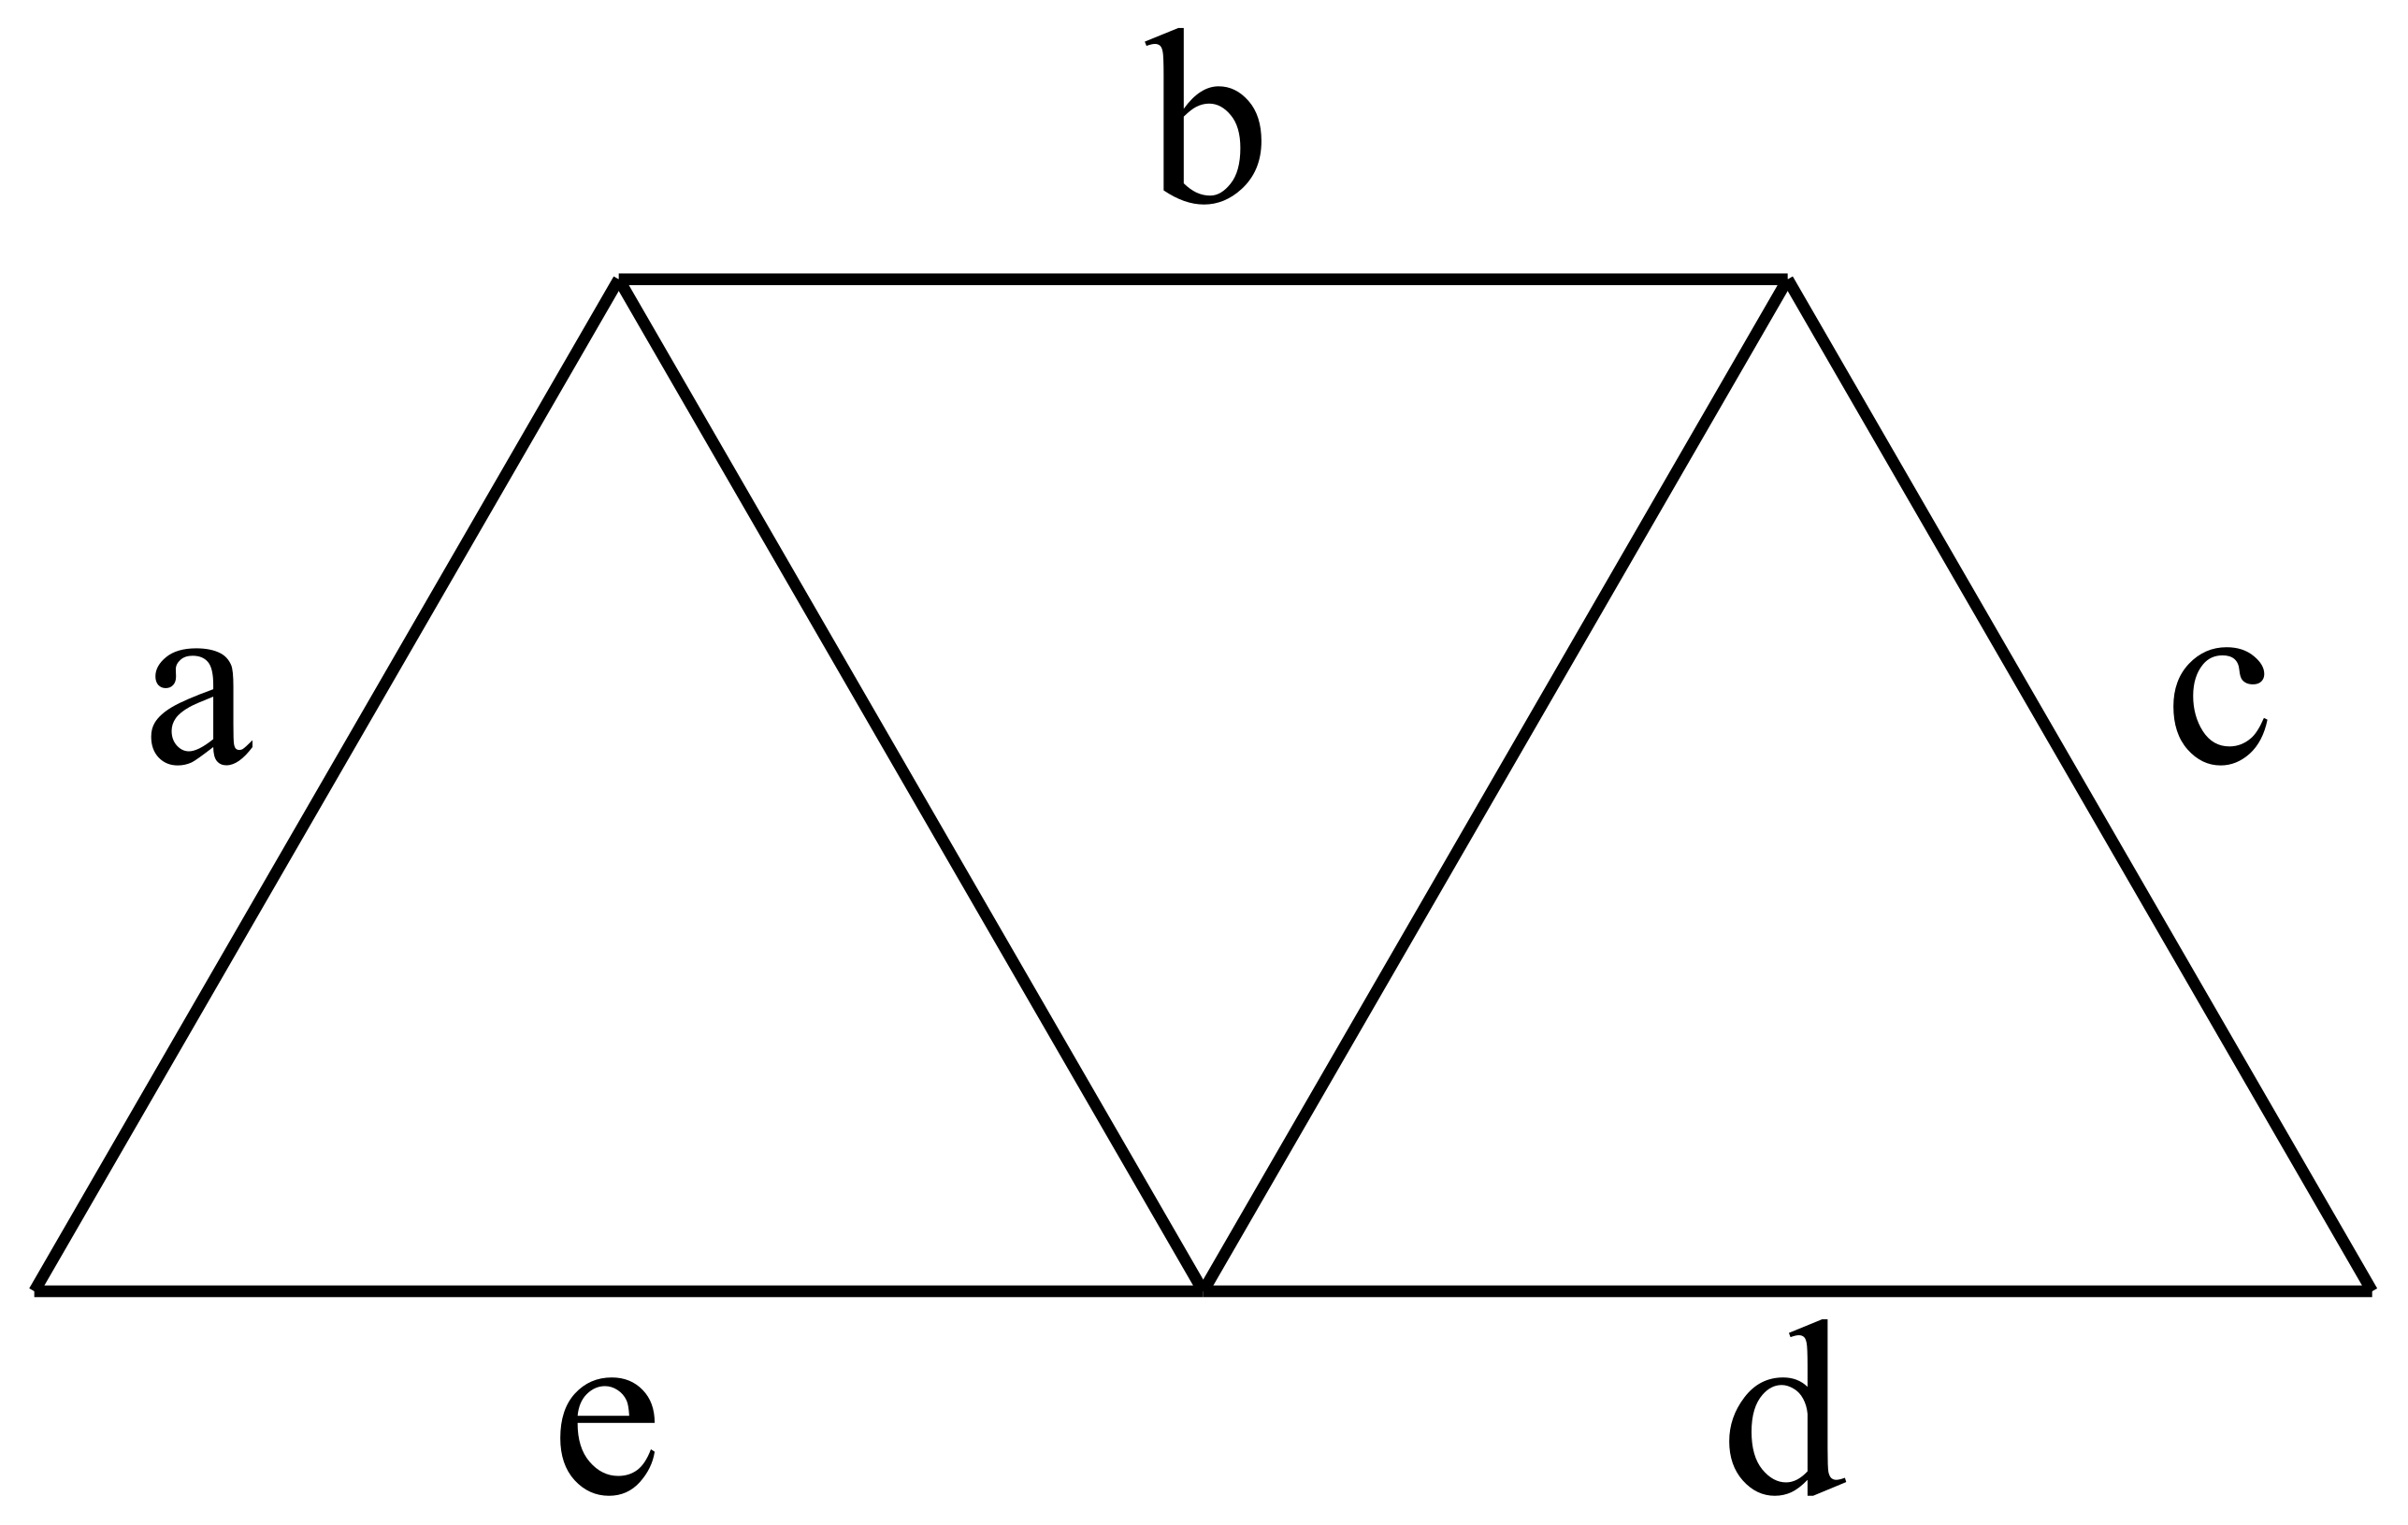
\includegraphics[width=1.5in]{triangles1.png}
\end{center}
\vspace{0.1in}

This shape has five edges where the last triangle can be attached.
I have labeled the edges a--e.
Although there are five edges, there are only three final shapes that can be made with the fourth triangle, which are shown here:

\vspace{0.1in}
\begin{center}
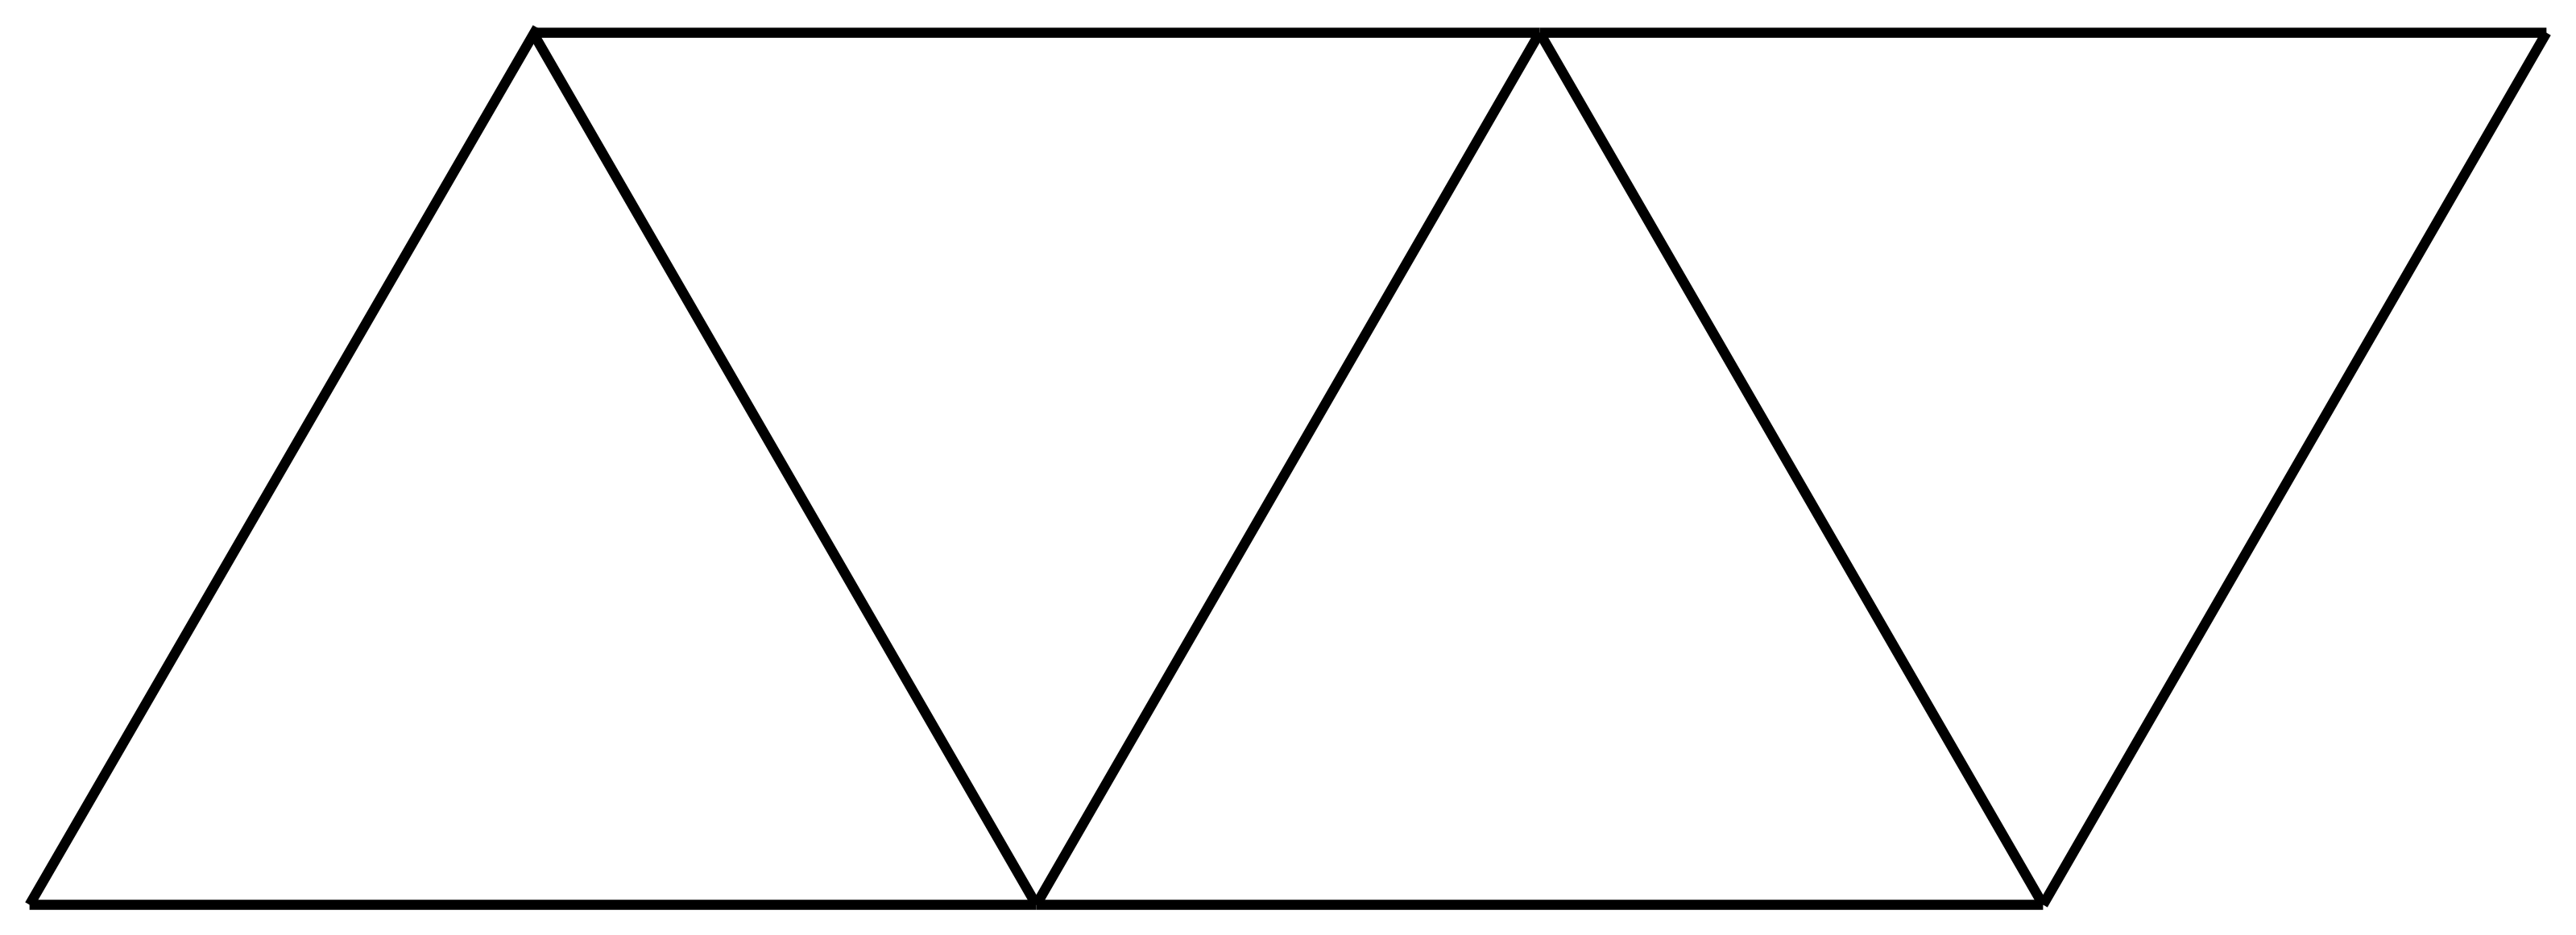
\includegraphics[width=1.863in]{triangles3.png}
\hspace{0.25in}
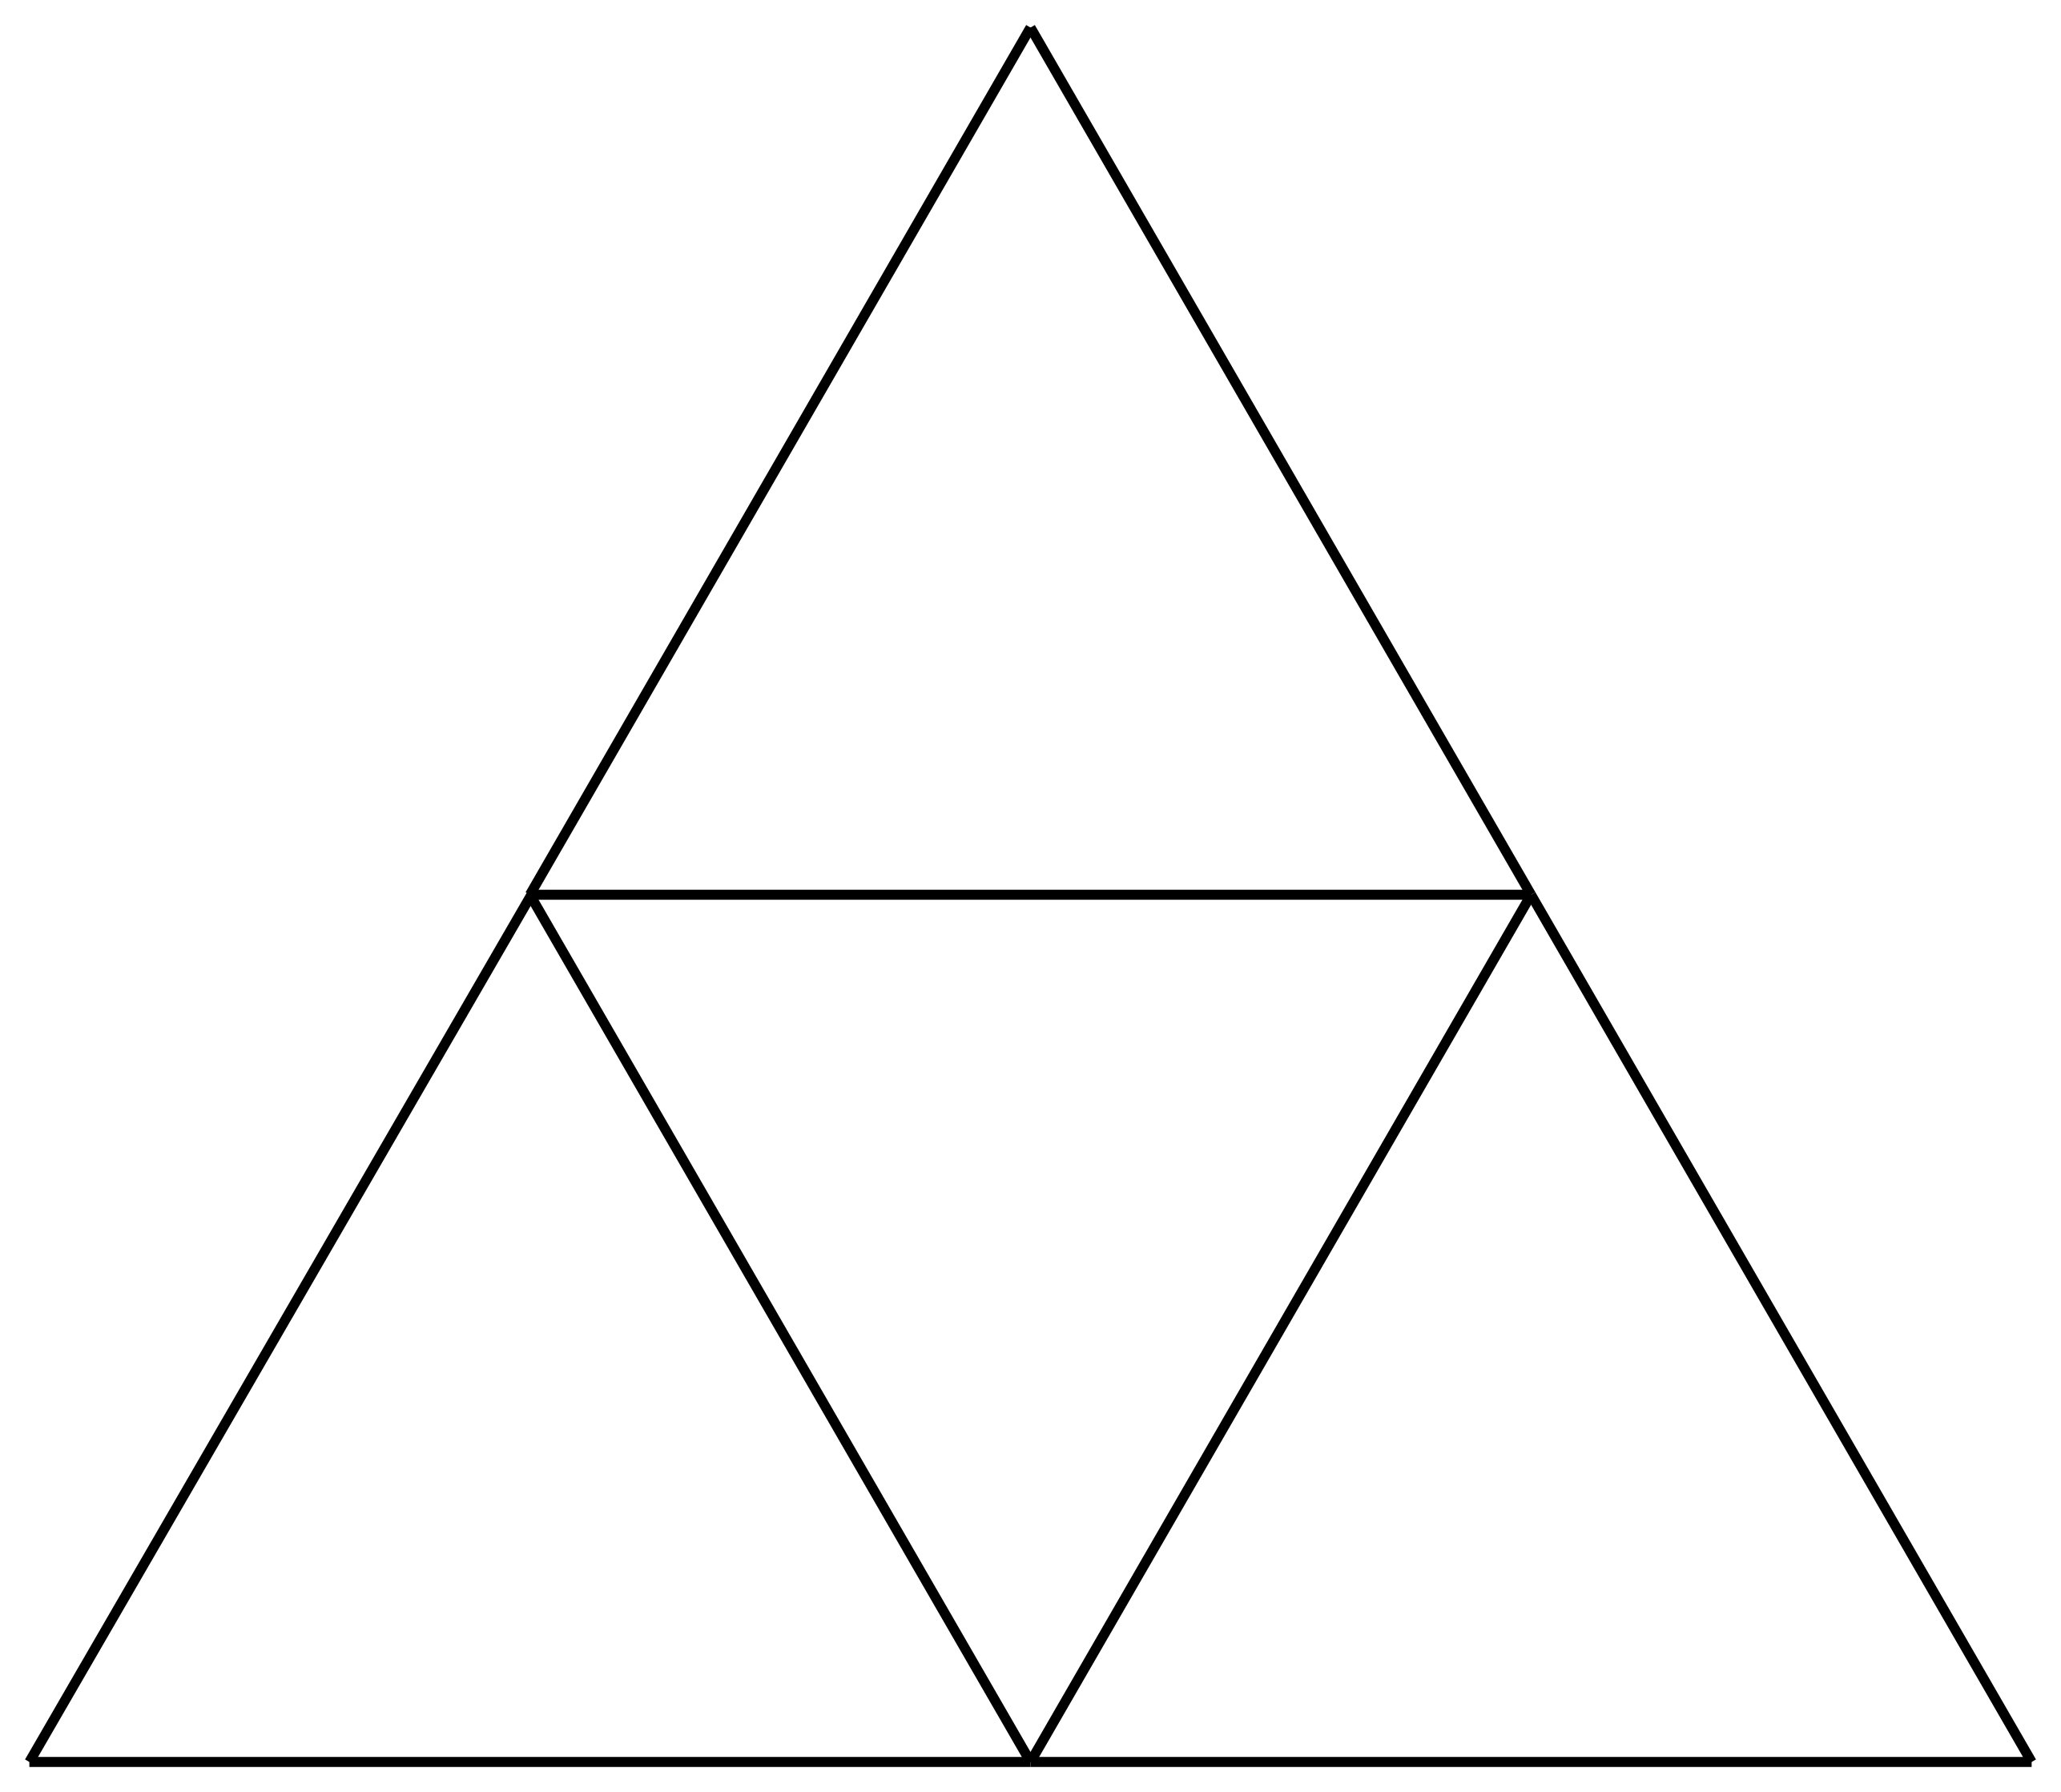
\includegraphics[width=1.5in]{triangles2.png}
\hspace{0.25in}
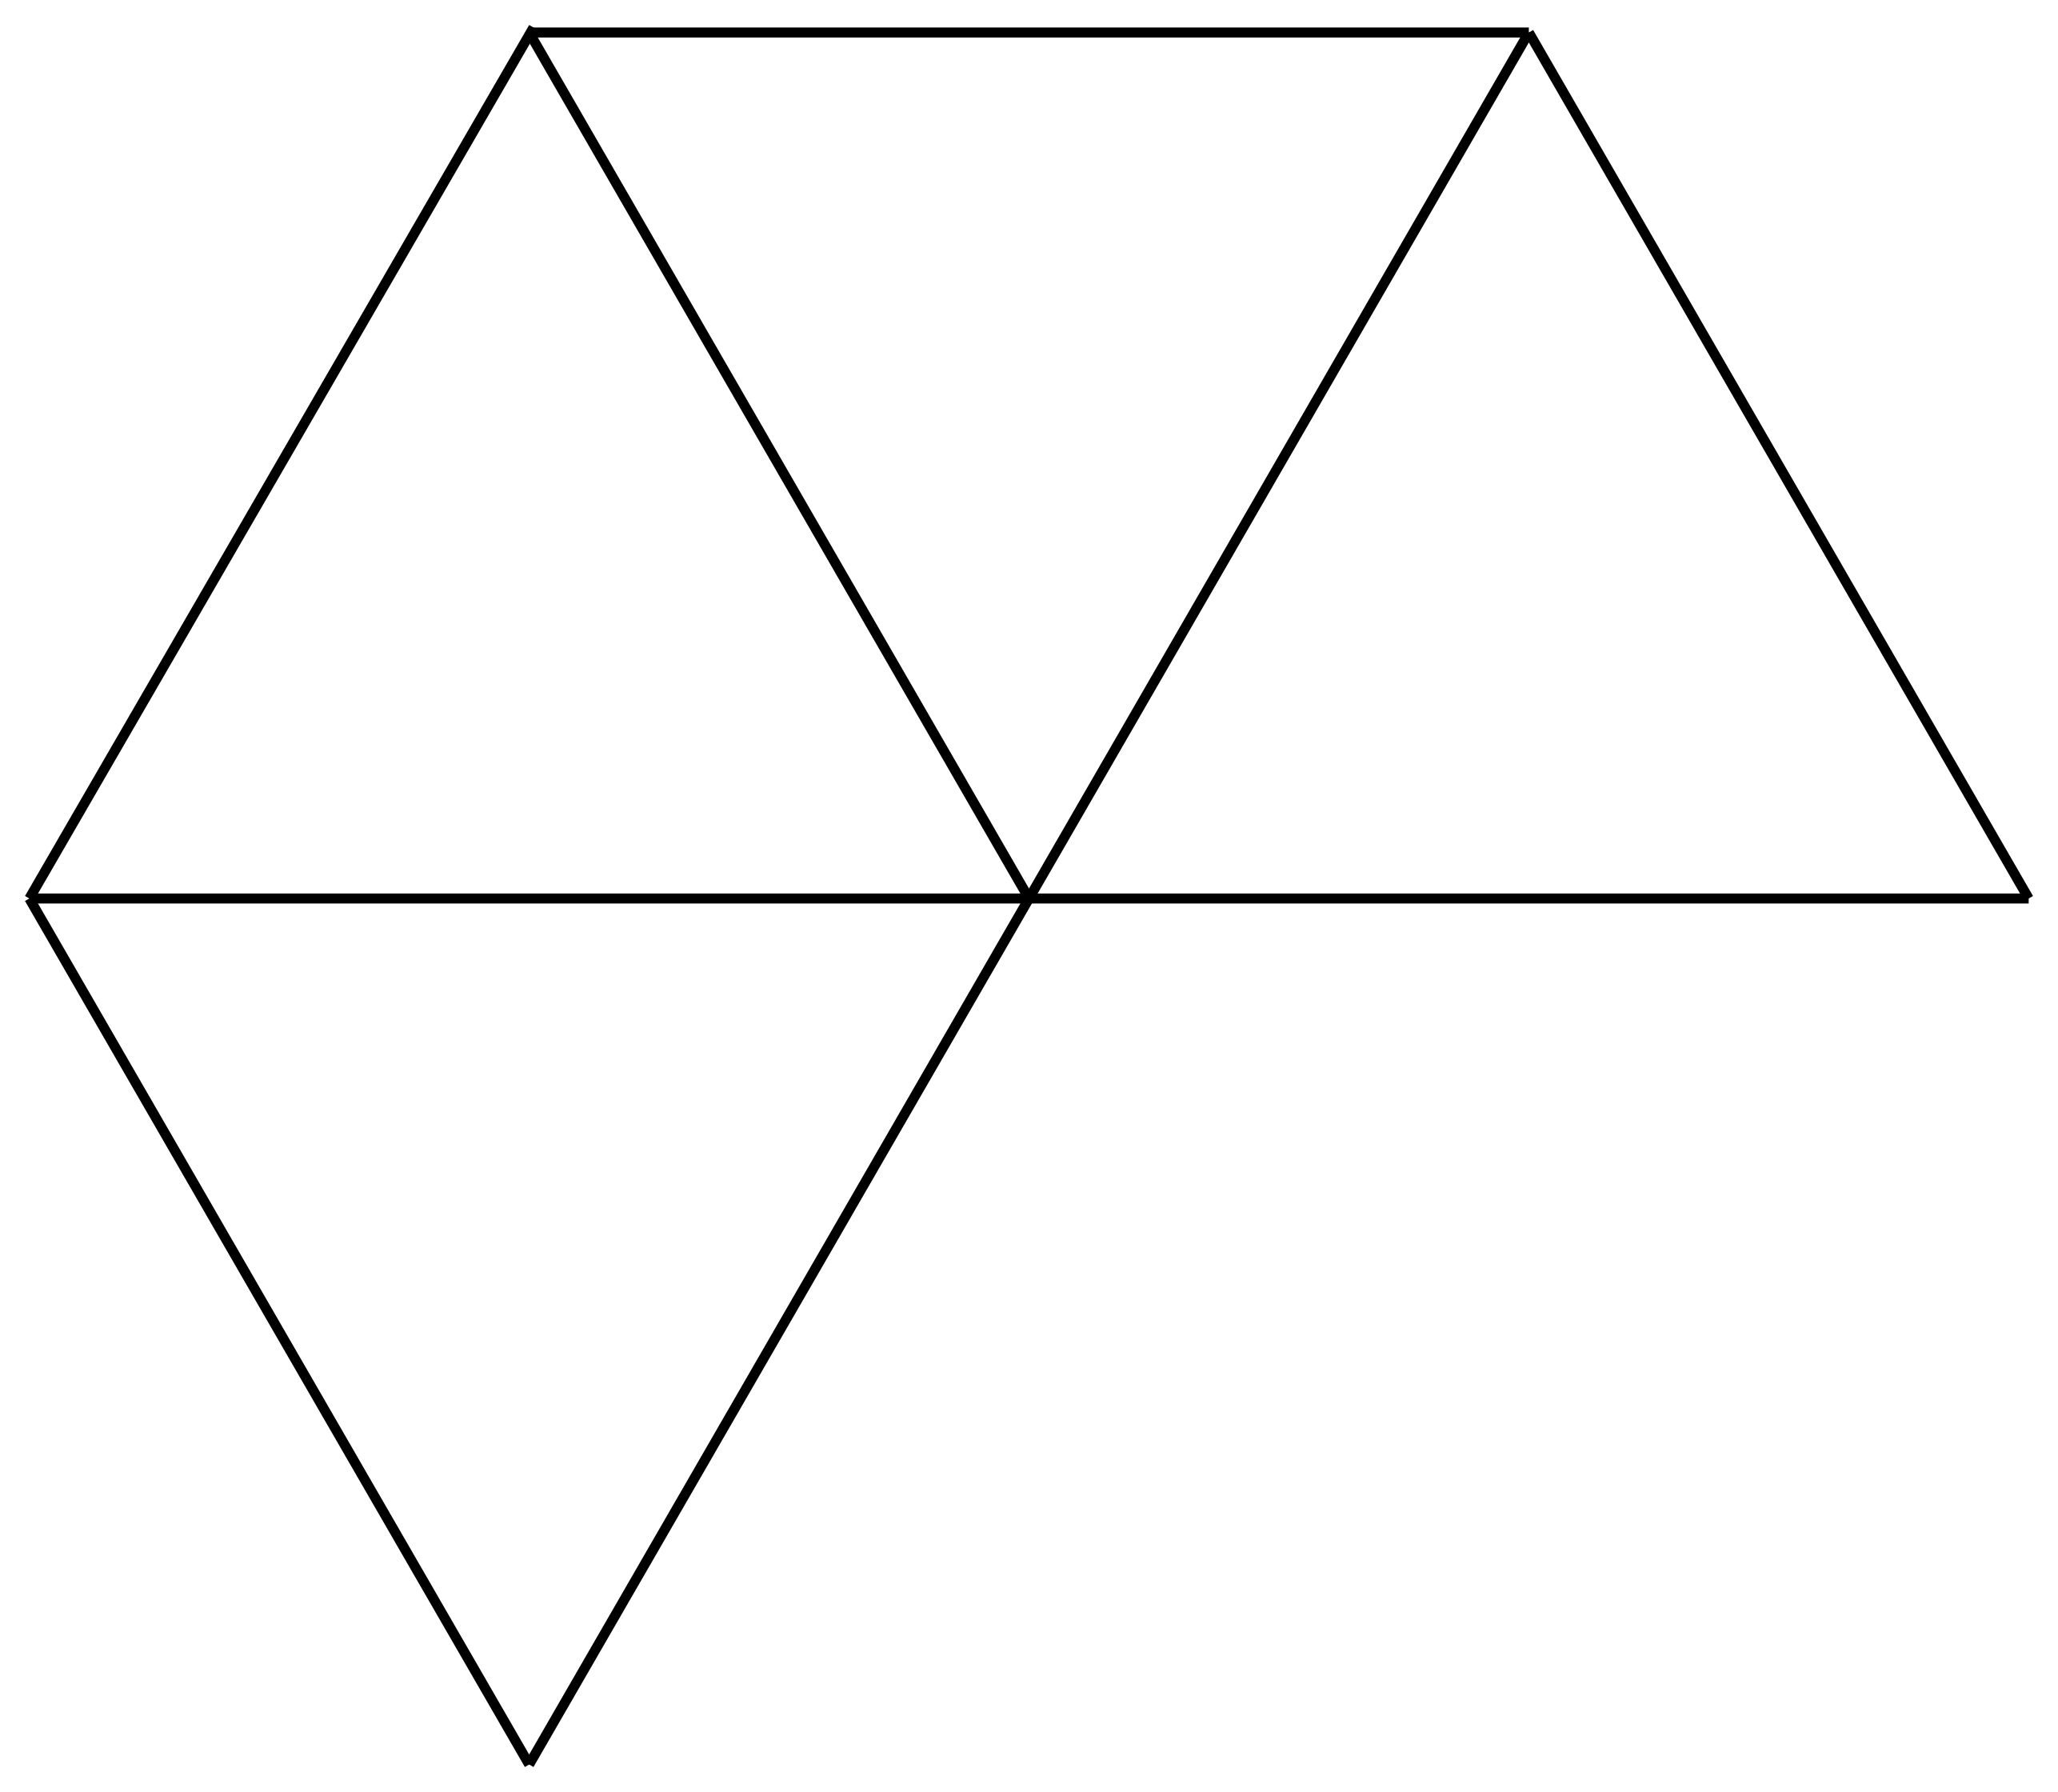
\includegraphics[width=1.5in]{triangles4.png}
\end{center}
\vspace{0.1in}

Attaching the last triangle at side a forms the mirror image of attaching at side c.
These both look like the shape on the left.
Attaching at side b forms the shape in the middle.
Attaching at side d or e forms the shape on the right.

Only the left and middle shapes can be folded into a tetrahedron.
Those constitute three of the five possible attachments.
Because each of the five edges is equally likely to be attached, the solution is
\fcolorbox{red}{white}{$\bm{{\nicefrac{3}{5}}}$}\,.

I decided to also attempt the problem of attaching squares to form a cube.
I listed out all possible ways to attach two, three, four, and five cubes.
My crude, not-to-scale, drawings are shown on the last page.

There is only one shape formed by attaching two squares.
For three squares, there are two shapes, which I have labeled 3a and 3b.
Four squares form five shapes (up to reflection), which are famous Tetris shapes (tetrominoes), and I have labeled 4a through 4e (in no particular order).
Five squares can form 12 different shapes, which I labeled 5a through 5l (again in no particular order).

The probabilities of forming the shapes are in general different and depend on how the squares are attached in order.
For example, shape 3a has eight edges, and can form shape 4a with probability \nicefrac{1}{4}, shape 4b with probability \nicefrac{1}{2}, or shape 4c with probability \nicefrac{1}{4}.
It is also important to notice which shapes cannot be further attached in any way to form a cube.
I call these shapes ``dead-ends''.
The dead-ends shown in my drawings are 4e, 5a, 5c, 5j, and 5k.
To determine the total probability of forming a cube-foldable shape, I have calculated the probability of creating each labeled shape, avoiding any previous dead-end in the path toward that shape.
I list these probabilities here:

\vspace{0.1in}
\begin{center}
\begin{tabular}{ccccccccccc}
Shape & Probability & & Shape & Probability & & Shape & Probability & & Shape & Probability \\
\cline{1-2} \cline{4-5} \cline{7-8} \cline {10-11}
2  & 1                & & 4c & \nicefrac{1}{4}  & & 5c & \nicefrac{7}{30}  & & 5h & \nicefrac{1}{15} \\
3a & \nicefrac{1}{3}  & & 4d & \nicefrac{1}{6}  & & 5d & \nicefrac{7}{120} & & 5i & \nicefrac{1}{30} \\
3b & \nicefrac{2}{3}  & & 4e & \nicefrac{1}{6}  & & 5e & \nicefrac{7}{60}  & & 5j & \nicefrac{1}{30} \\
4a & \nicefrac{1}{12} & & 5a & \nicefrac{1}{60} & & 5f & \nicefrac{1}{40}  & & 5k & \nicefrac{1}{30} \\
4b & \nicefrac{1}{3}  & & 5b & \nicefrac{1}{15} & & 5g & \nicefrac{7}{60}  & & 5l & \nicefrac{1}{30} \\
\end{tabular}
\end{center}
\vspace{0.1in}

The total probability of creating a five-square shape that is not a dead-end is \nicefrac{31}{60}.
From here, it is easy to calculate the probability of attaching the last square to form a cube-foldable shape.
Each  five-square shape has a total of 12 edges.
If the five squares are folded to form a cube that is just missing a single side, then there are four edges which surround that missing side.
That means there are just four edges in the original un-folded shape which will create a valid six-square shape.
Thus as long as the first five squares form a valid shape, there is a probability of $\nicefrac{4}{12}=\nicefrac{1}{3}$ of ending up with a valid six-square shape.
So the answer to the first part of the extra credit problem is $\nicefrac{31}{60}\times\nicefrac{1}{3}$, or
\fcolorbox{red}{white}{$\bm{{\nicefrac{31}{180}}}$}\,.

I have not attempted any of the other Platonic solids.

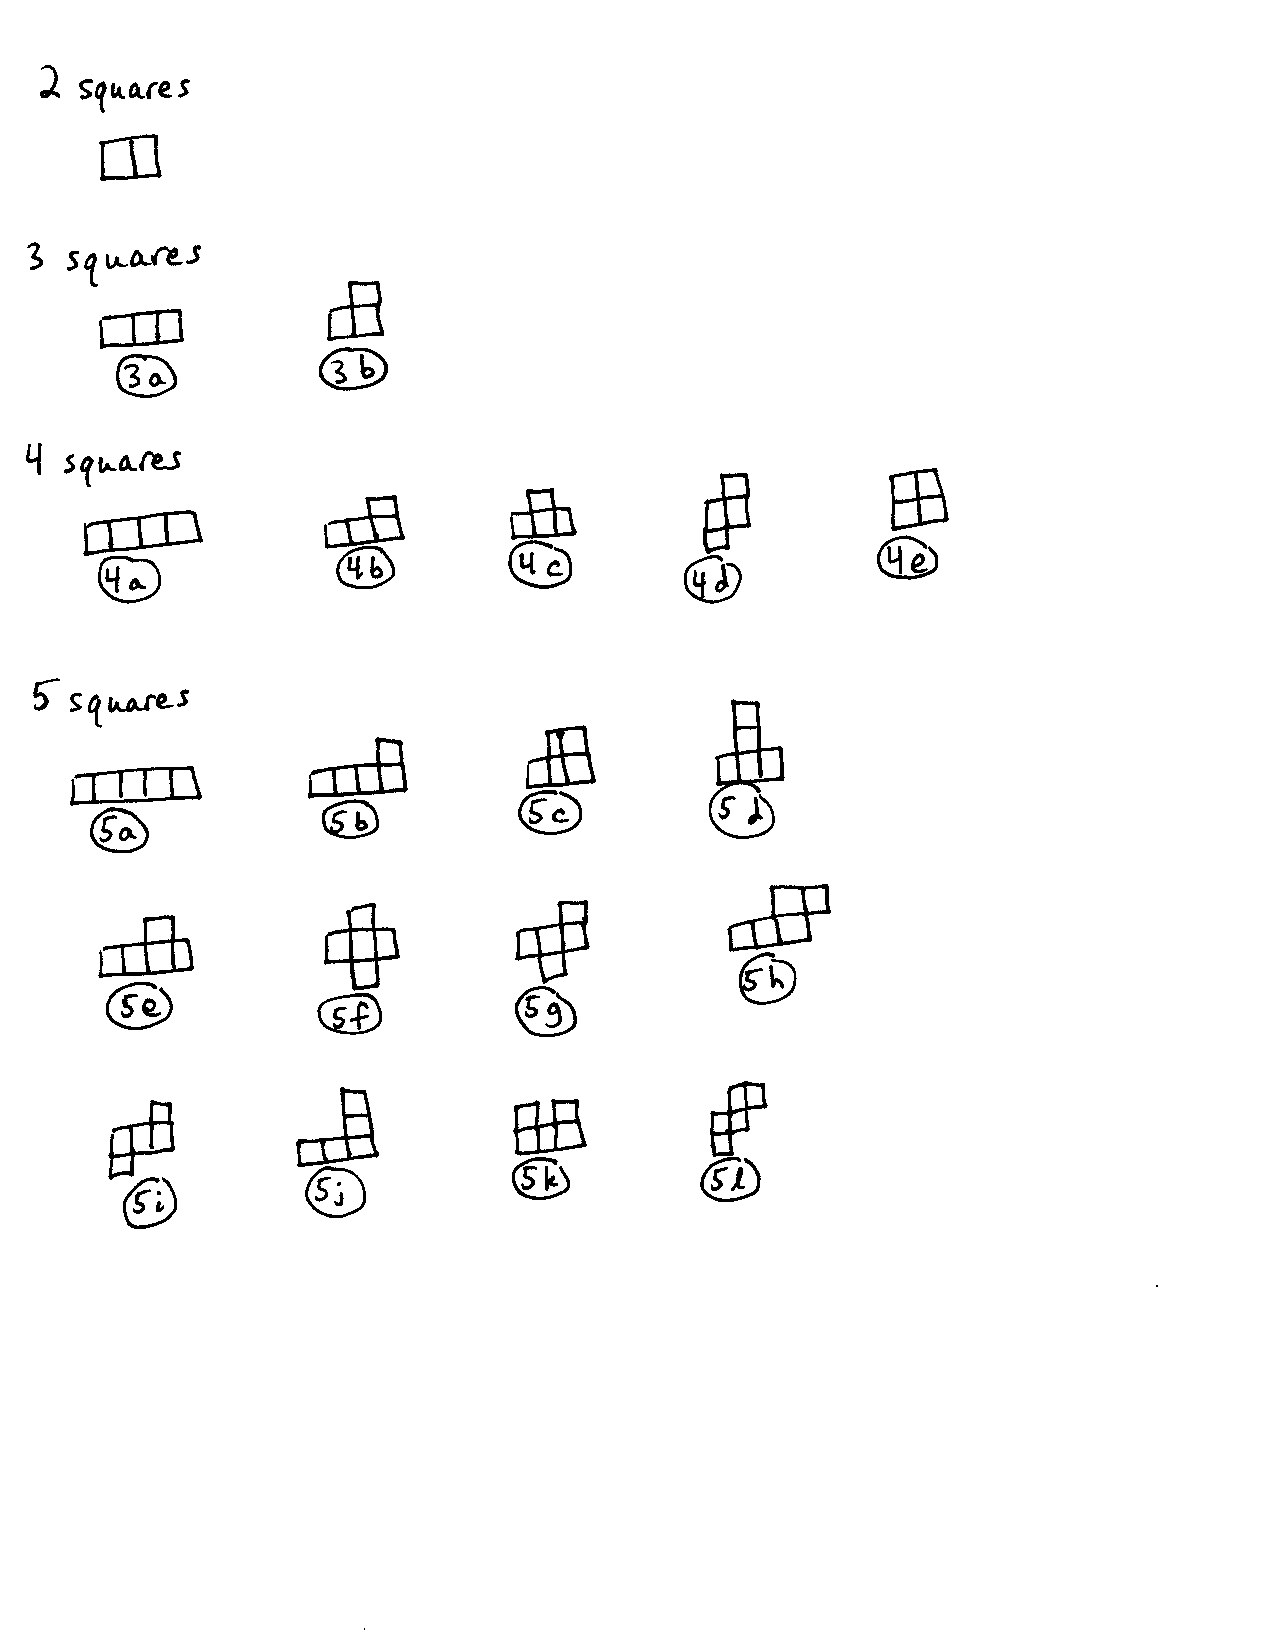
\includepdf{squares.pdf}



\end{document}